\documentclass[12pt]{article}

\usepackage[english]{babel}
\usepackage[english]{isodate}
\usepackage[table,svgnames]{xcolor}
\usepackage{url}
\usepackage[utf8x]{inputenc}
\usepackage[T1]{fontenc}
\usepackage{longtable}
\usepackage{amsmath}
\usepackage{graphicx}
\usepackage{parskip}
\usepackage{fancyhdr}
\usepackage{vmargin}
\usepackage{hyperref}
\usepackage{pgfgantt}
\usepackage{pgf-umlcd}
\usepackage{xparse}
\usepackage{float}
\usepackage{tabularx}
\usepackage{titling}
\usepackage{fancyhdr}
\usepackage{rotating}
\usepackage{lscape}

% Global graphiscspath
\graphicspath{{../../../img/}}

% Styling changes

%% Better margins
%\setmarginsrb{1 cm}{1 cm}{1 cm}{1 cm}{0 cm}{0 cm}{0 cm}{0 cm}

\begin{document}
	\pagestyle{empty}

	\begin{figure}[ht]
  		\centering
	  	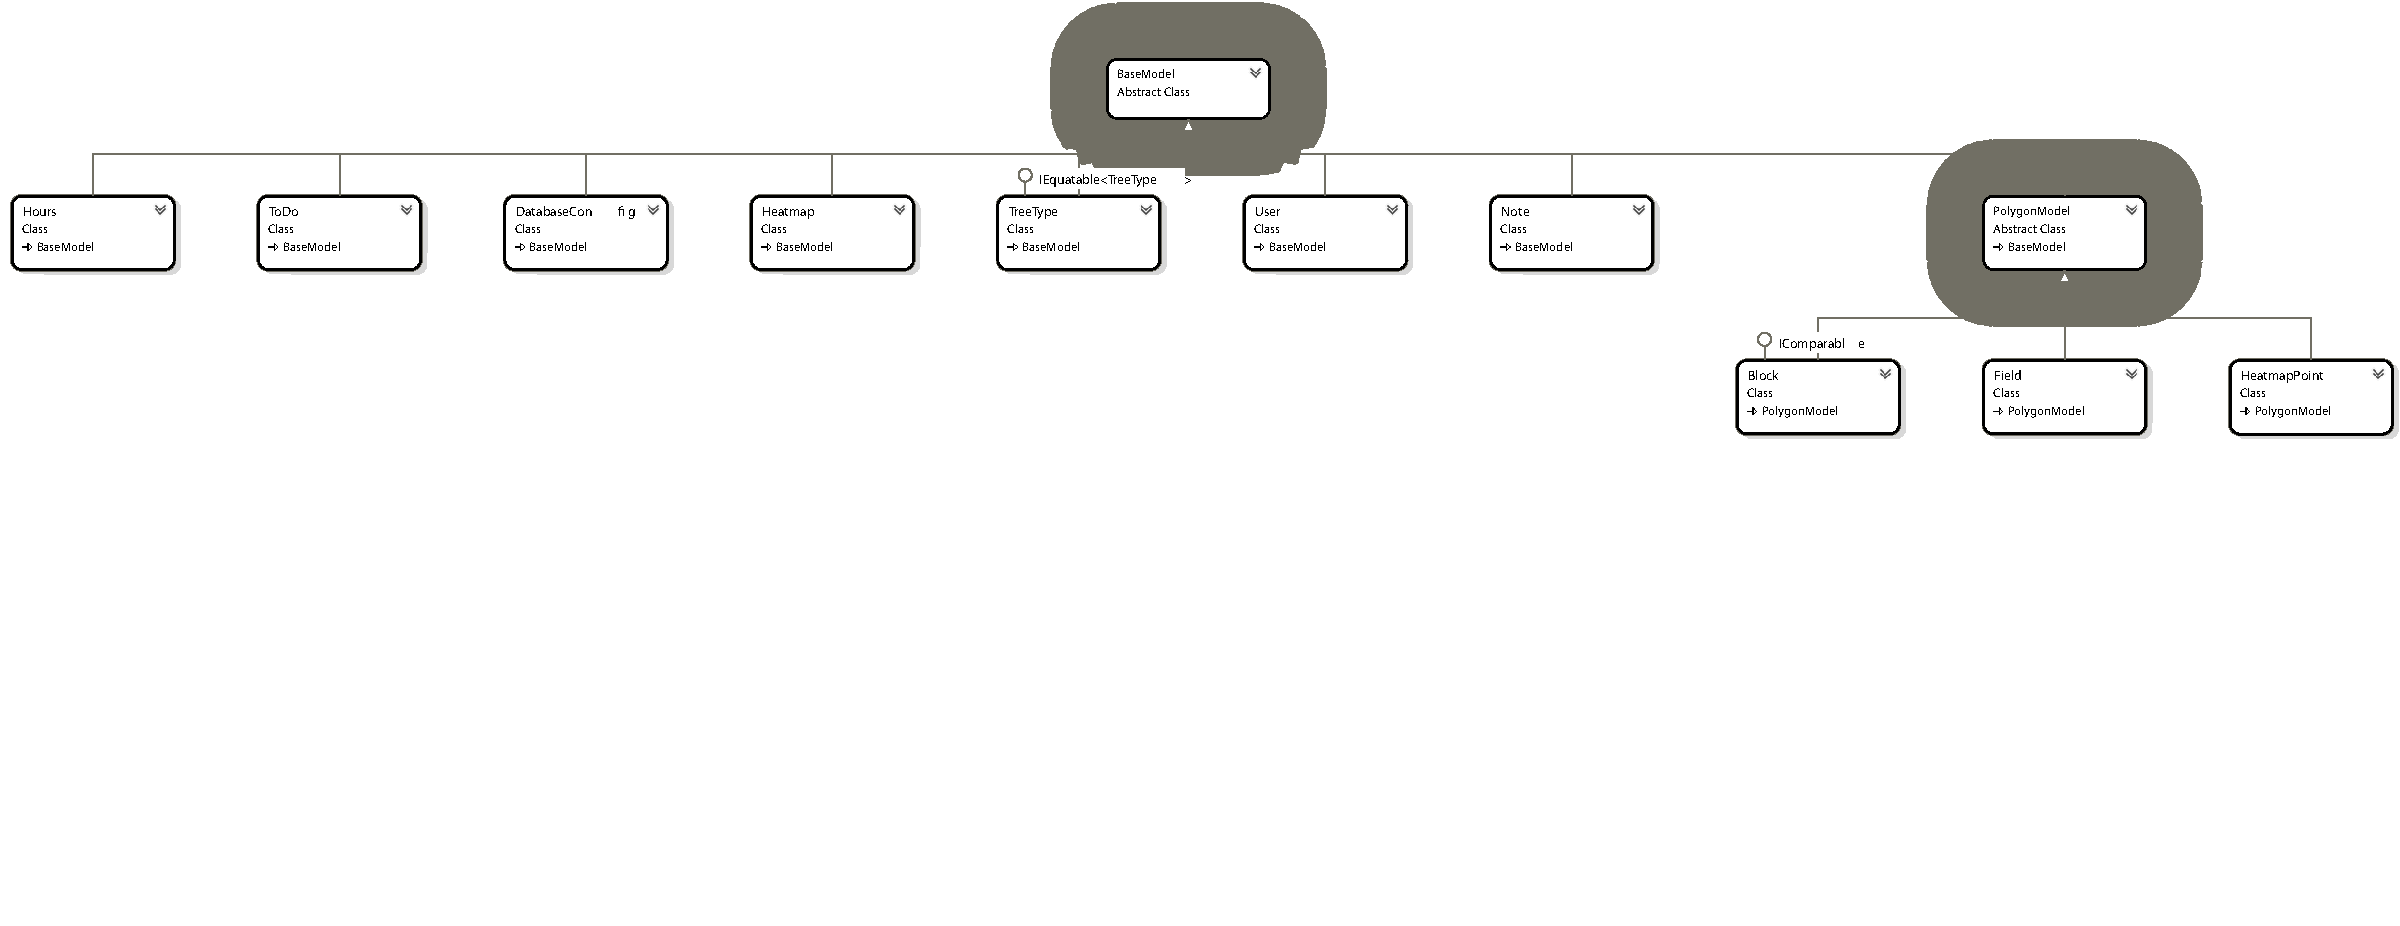
\includegraphics[width=\textheight,keepaspectratio,angle=90]{ClassDiagram1-part1.pdf}
	  	\caption{Class Diagramm Forms Part 1\label{fig:ClassDiagramPart1}}
	\end{figure}

	\begin{figure}[ht]
	  	\centering
	  	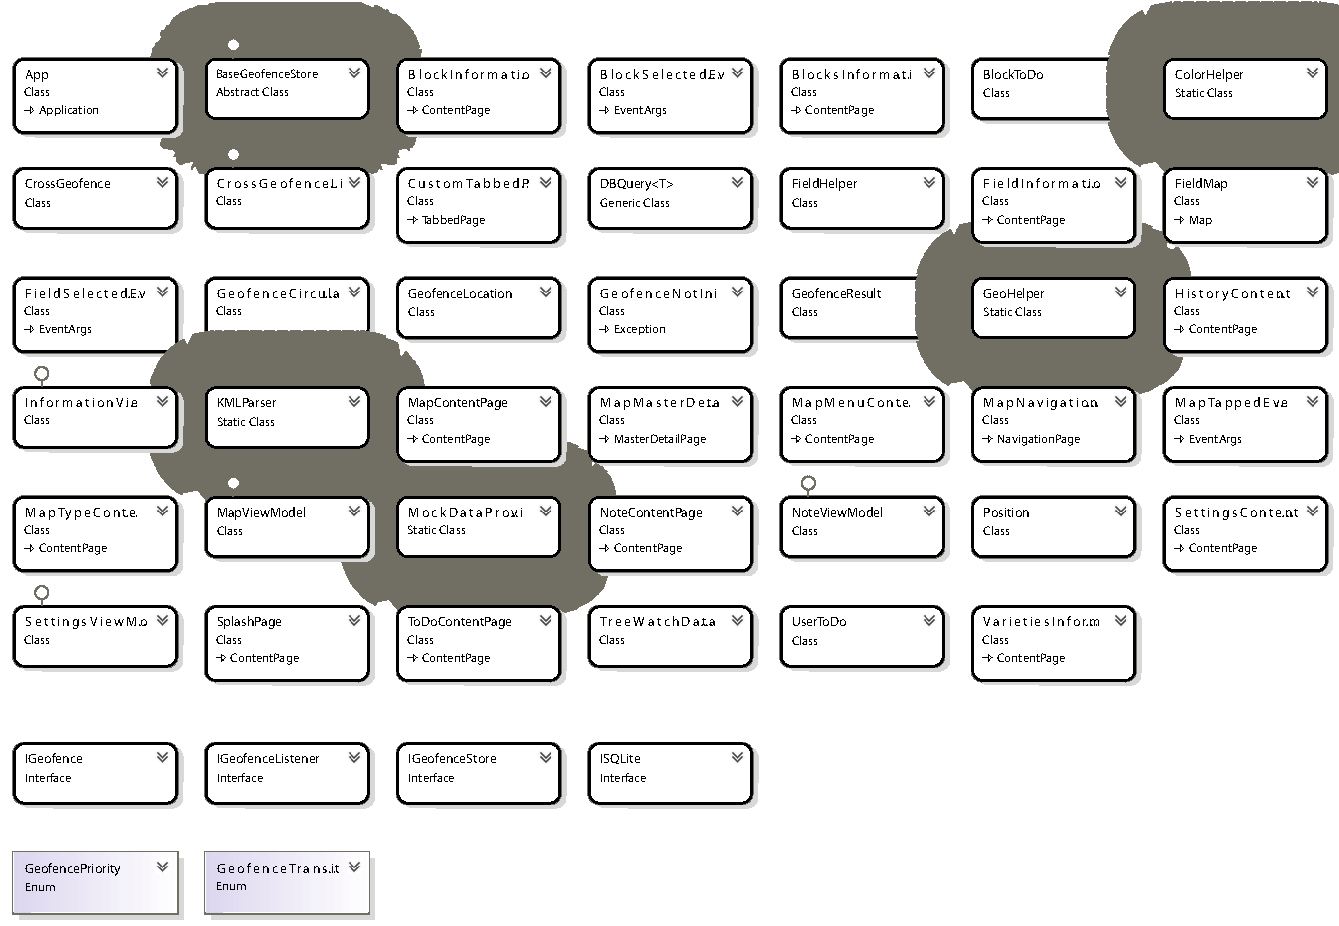
\includegraphics[width=\textheight,keepaspectratio,angle=90]{ClassDiagram1-part2.pdf}
	  	\caption{Class Diagramm Forms Part 2\label{fig:ClassDiagramPart2}}
	\end{figure}
  
  \clearpage

	\begin{figure}[ht]
	  	\centering
	  	
\includegraphics[width=\textheight,keepaspectratio,angle=90]{ClassDiagramiOS.pdf}
	  	\caption{Class Diagramm iOS\label{fig:ClassDiagramIos}}
	\end{figure}

	\begin{figure}[ht]
		\centering
	  	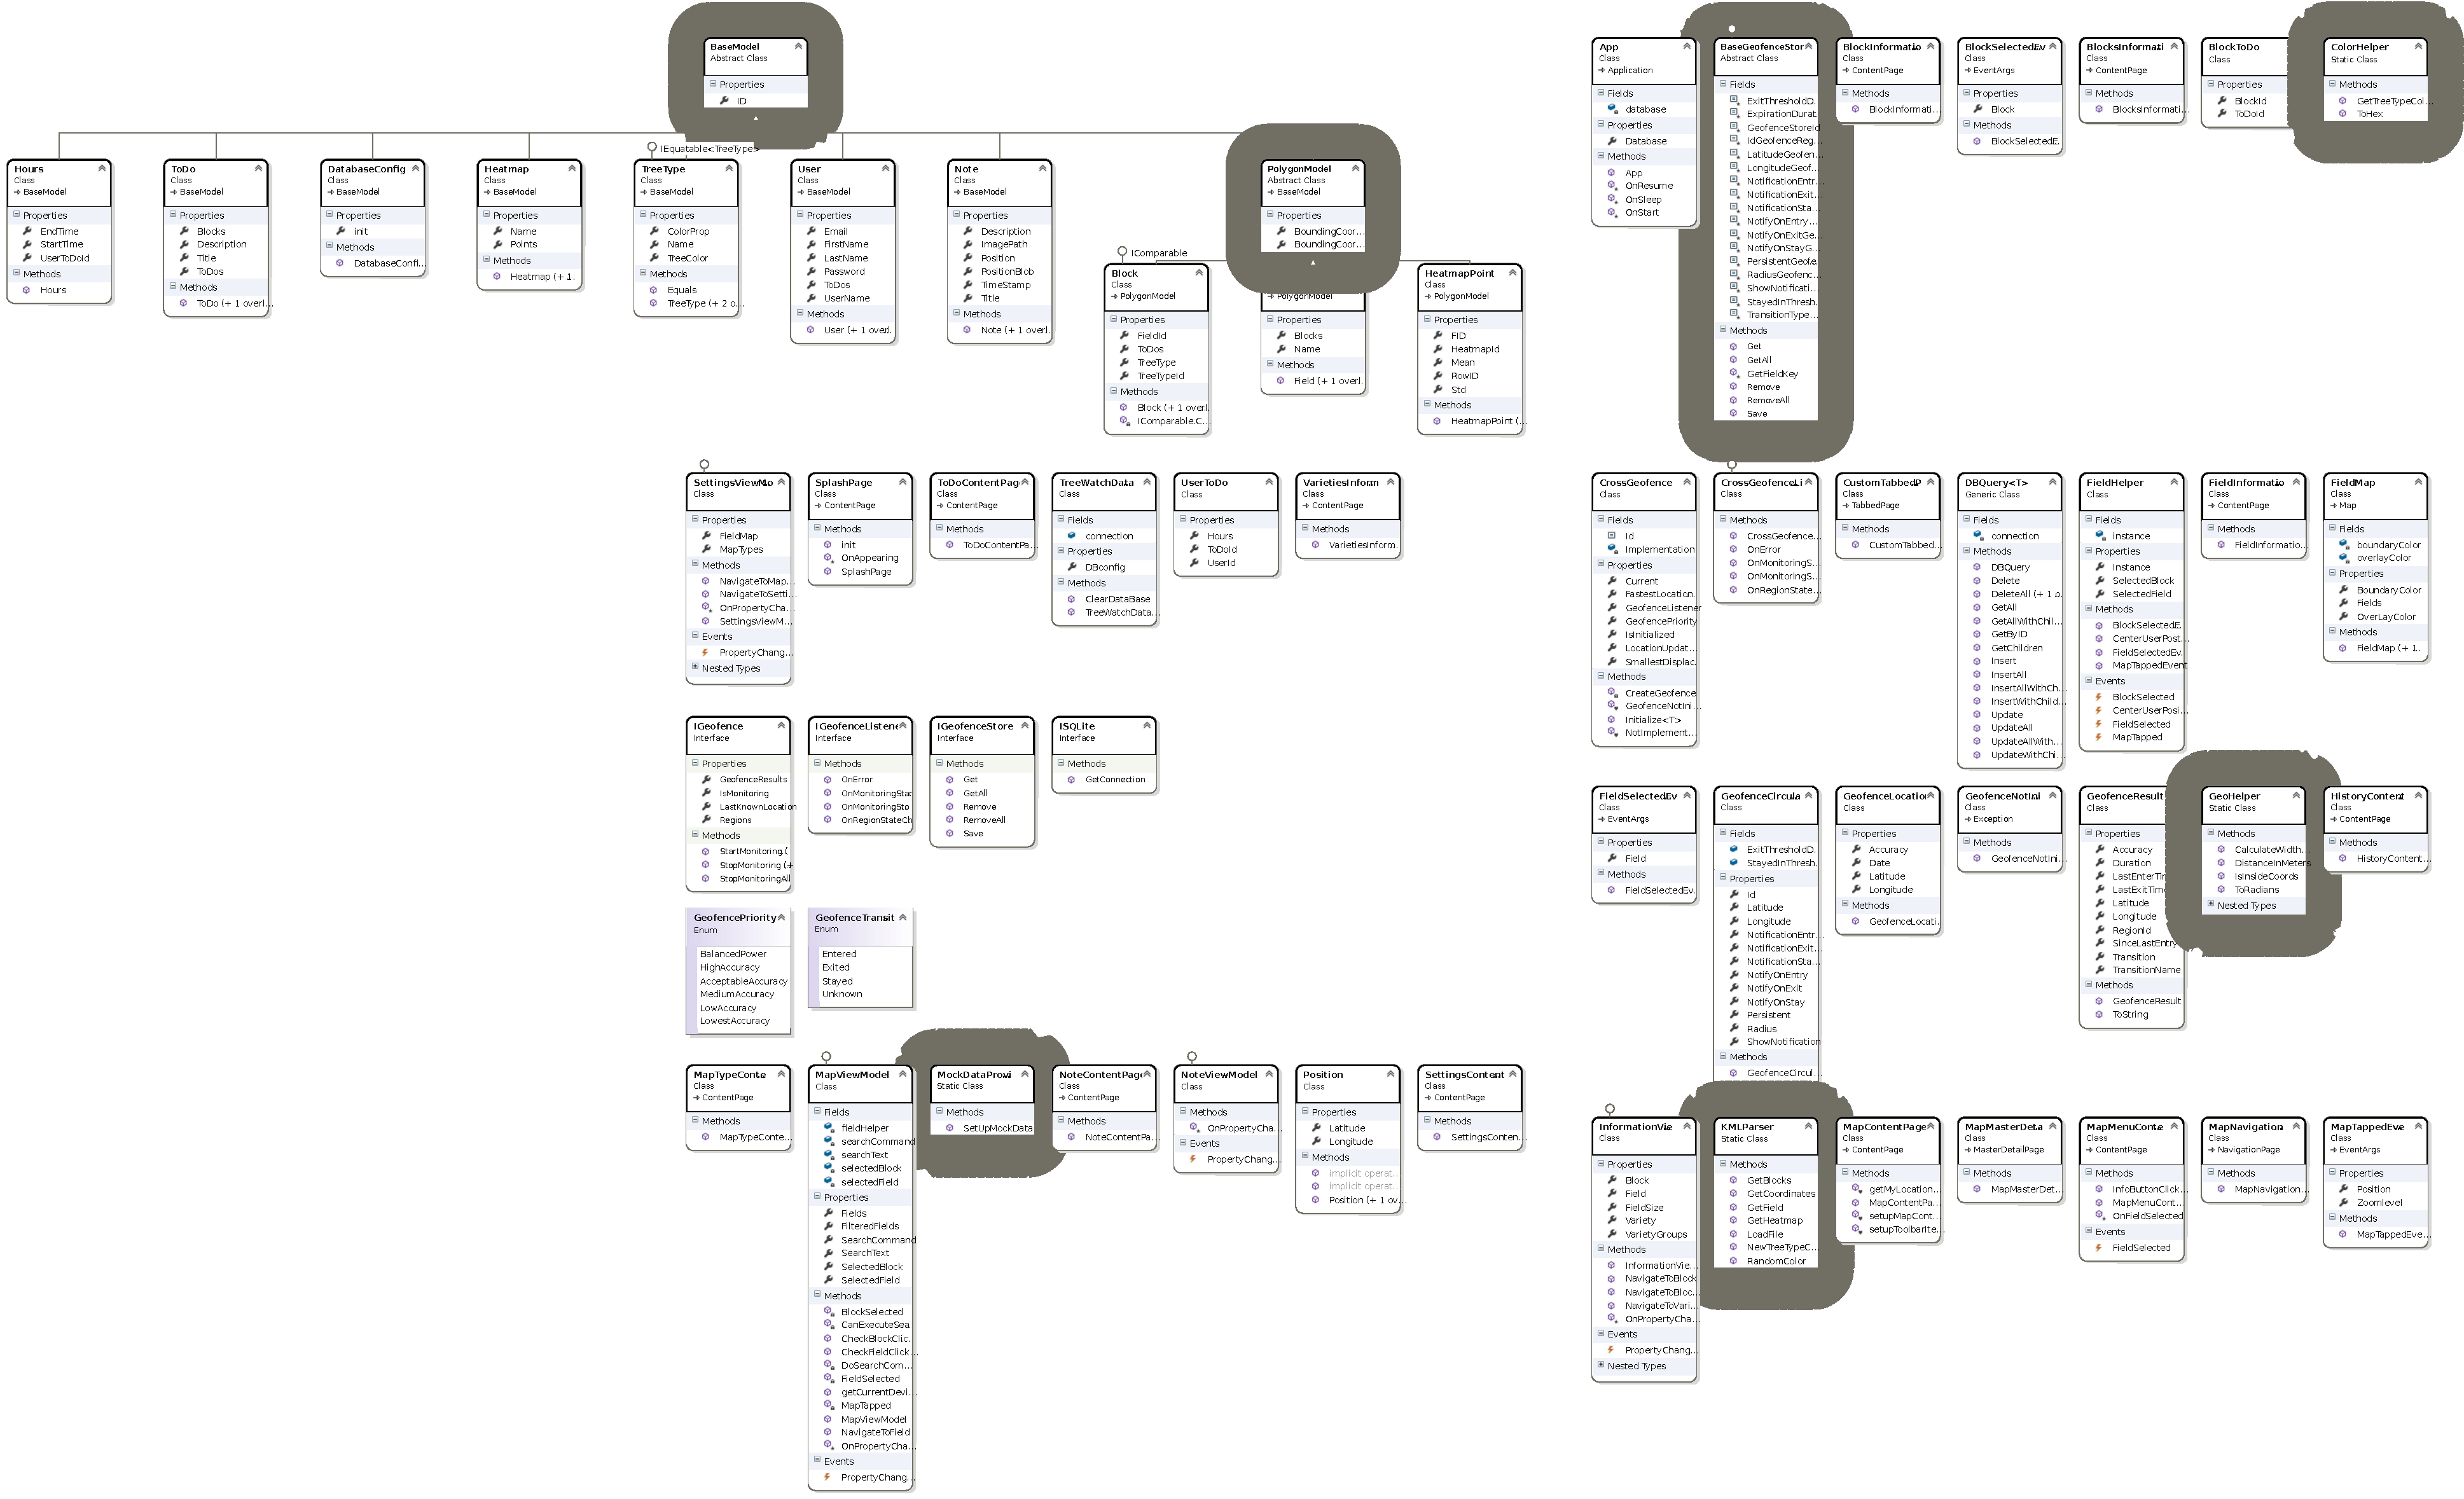
\includegraphics[width=\textheight,keepaspectratio,angle=90]{ClassDiagramForms.pdf}
	  	\caption{Class Diagramm Forms\label{fig:ClassDiagramForms}}
	\end{figure}

\end{document}